\documentclass[12pt]{zettel}

\usepackage{booktabs}

\usepackage{geometry}
\geometry{tmargin=2cm,bmargin=2cm,lmargin=3cm,rmargin=3cm}

\renewcommand{\gregor}{\put(13.2,-3.0){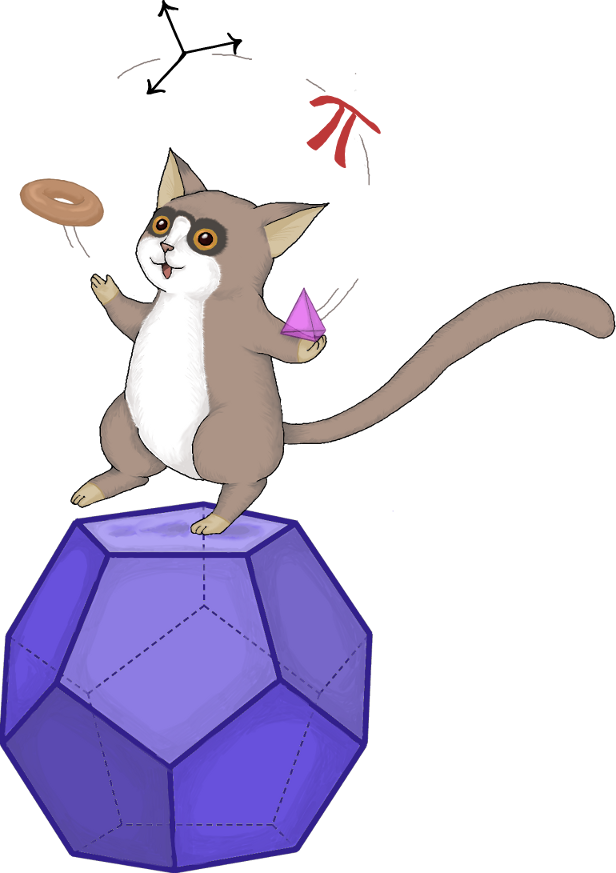
\includegraphics[scale=0.18]{cover}}}

\usepackage{framed}
\definecolor{shadecolor}{rgb}{.97,.97,.97}

\begin{document}

\renewcommand{\betreff}{}

\makeletterhead{}

\vspace{-2em}

\begin{center}
  \Large\textbf{\textsf{Bewerbung um den Witty-Förderpreis 2014: \\
  Matheschülerzirkel Augsburg }}
\end{center}

Aus der Anforderungsbeschreibung: "`Das Projekt soll
Kindern/Jugendlichen Selbstwertgefühl vermitteln, sie fördern und nachhaltig
Hilfe zur Selbsthilfe bieten."'

\begin{itemize}
\item Information über Verein und Aktivitäten inkl. evtl. Presseberichte
\item Wie setzen sich die rd. 50 TeilnehmerInnen am Mathematikcamp zusammen? Kann
man sich einfach bewerben - läuft es über Lehrer bzw. Schulen?
\item Wie sieht es mit der "`Nachhaltigkeit"' aus? d.h. wie geht es weiter, wenn
einzelne Schüler richtig +Feuer fangen und Begabung zeigen?
\item Wie lauten Ihre Ziele bei diesen Aktivitäten und Projekten? Gibt es zu
wenig Mathematikstudenten und setzen Sie deshalb bereits so früh an?
\item Das Preisgeld beträgt 10.000 Euro. Für das Camp benötigen Sie 7000,--. Wie
würden Sie das restliche Preisgeld sinnvoll verwenden?
\end{itemize}

\section{Bewerber}

Wir sind Doktoranden und Mitarbeiter des Instituts für Mathematik der
Universität Augsburg.

Kurzvorstellung

Zielsetzung


\section{Projektbeschreibung}

Wofür soll das Preisgeld eingesetzt werden?

Was macht das Projekt einmalig/einzigartig für unsere Region?


\section{Vision}

Das Hauptziel des Mathezirkel Augsburg ist es, Schülerinnen und Schülern
langfristig eine Möglichkeit zu bieten, ihrem Interesse an der
Mathematik nachzugehen. Wir wollen Kindern, die frühzeitig Spaß an der
Mathematik haben, dazu animieren und darin unterstützen, an ihrem
Interesse festzuhalten. Es geht uns darum, diesen Schülerinnen und
Schülern zu zeigen, was man mit Mathematik alles Spannende machen kann
und wie diese außerhalb der Schule aussieht. Langfristig hoffen wir,
dass sich die Jugendlichen durch eine ernsthafte Beschäftigung mit der
Mathematik darüber klar werden, was sie im Leben wollen und dann auf
ihrem Weg auch Mittel und Ideen der Mathematik anwenden können. Dabei
ist uns nicht wichtig, dass sie später Mathematik studieren, sondern
vielmehr, dass sie die Mathematik nicht für etwas Gefährliches halten
und sie stattdessen die Mathematik in ihrem Leben benutzen können.

Viele Beschäftigungen von Schülerinnen und Schülern neben der Schule
werden von der Gesellschaft als normal wahrgenommen, die Mathematik
gehört jedoch leider nicht dazu. Wir hoffen, dass wir einen Beitrag dazu
leisten können, zur Aktzeptanz der Mathematik in der Öffentlichkeit
beizutragen und damit auch mathematisch interessierten Jugendlichen zu
helfen.

Ein wichtiger Punkt auf dem Weg zum Erhalt des Interesses an der
Mathematik, welcher auch für sich selbst bereits erstrebenswert ist, ist
das Zusammenbringen von Schülerinnen und Schülern mit dem gemeinsamen
Spaß an der Mathematik. An einer einzigen Schule finden sich vielleicht
nur ein oder zwei Jugendliche, im Augsburg und Schwaben sind es jedoch
deutlich mehr. Durch regelmäßige Treffen und Ferienlager lernen die
Kinder Gleichgesinnte kennen, was ihnen enorm viel Spaß bereiten kann.
Wir hoffen, dass diese Begegnungen ihnen in ihrem weiteren Leben sehr
viel geben können.


\section{Zielgruppe(n)}

Unser Projekt richtet sich an mathematisch interessierte Schülerinnen
und Schüler der Klassenstufen 5 bis 12. Die einzige Voraussetzung zur
Teilnahme ist Spaß und Interesse an der Mathematik, es gibt insbesondere
keine Noten, Schulzugehörigkeiten oder Wettbewerbsergebnisse als
Beschränkung. Einerseits wollen wir sicherstellen, dass wir keine
Interessierten abschrecken und andererseits kann Spaß an der Mathematik
durchaus unabhängig sein von Schulergebnissen oder der Teilnahme an
Wettbewerben. Daher haben wir zum Anfang potentielle Teilnehmerinnen und
Teilnehmer durch Zeitungsartikel und Werbung an verschiedenen Schulen
geworben.

Im letzten Jahr haben wir gesehen, dass die meisten unserer Kinder eine
sehr hohe Motivation für Mathematik mitbringen und neugierig auf die
Mathematik außerhalb der Schule sind. Alle Jugendliche, die Interesse an
Rätseln, Logik und abstraktem Denken mitbringen, bilden unsere
Zielgruppe. Um die Kinder nicht durch Organisationsaufwand abzuschrecken
läuft die Anmeldung sehr unbürokratisch -- insbesondere kann jederzeit
eingestiegen werden.

Es hat sich gezeigt, dass auch wenn der Großteil unser Schülerinnen und
Schüler Gymnasien besucht, dennoch einige Realschülerinnen teilnehmen.
Wir haben auch bei Berufsschulen geworben, wo wir auch durch eine
engagierte Lehrerin vor Ort unterstützt wurden, leider stieß unser
Angebot dort aber auf kein Interesse. Wir versuchen im nächsten
Schuljahr durch noch breitere Öffentlichkeitsarbeit und Kontaktieren von
z.B. Realschulen, auch diesen Jugendlichen unser Angebot besser bekannt
zu machen.

Bis auf wenige Viertklässler sind alle unsere Teilnehmerinnen und
Teilnehmer in der fünften bis zwölften Klasse, wobei die niedrigeren
Klassenstufen einen größeren Anteil annehmen. Dies deckt sich mit der
Erfahrung von anderen Orten, dass anfangs ein größeres Interesse für
Mathematik vorherrscht und sich dieses oft im Laufe der Pubertät
auflöst, ein Problem, das wir versuchen gezielt zu lösen. Konkret haben
wir insgesamt 250 Schülerinnen und Schüler, davon in Klasse 5, in Klasse
6, in Klasse 7, in Klasse 8, in Klasse 9, in Klasse 10, in Klasse 11 und
in Klasse 12.

Ein weiteres bekanntes Problem der Naturwissenschaften im Allgemeinen
und der Mathematik im Speziellen ist der niedrige Frauenanteil in der
Oberstufe und im Studium. Tatsächlich zeigt die Erfahrung sowohl in
Augsburg als auch an anderen Orten, dass der Jungen- und Mädchenanteil
in den Klassenstufen Fünf und Sechs noch recht ausgeglichen ist. Wir
versuchen ganz gezielt durch konkrete Ansätze wie zum Beispiel XXXXX
diese Mädchen weiterhin für Mathematik zu begeistern.


\section{Budget}

Wir selbst arbeiten ehrenamtlich. Finanzielle Unterstützung benötigen wir aber
für die Veranstaltungen, die wir durchführen. Die größte Posten nehmen dabei das
Mathecamp (7.000,--~\texteuro) und die Durchführung der XXXten Stufte der
Mathematik-Olympiade ein (2.000,--~\texteuro). Materialien für die
Zirkelarbeit, Preise für Schülerinnen und Schüler und die Durchführung von
Abschluss- und Auftaktveranstaltungen kosten etwa 1.000,--~\texteuro.

Der Universität gilt insofern Dank, als dass wir unentgeltlich ihre
Räumlichkeiten nutzen können und Büromaterialien, Briefporto und ähnliche
Posten über sie abwickeln können.

Nachstehend unsere detaillierte Kalkulation. Möglicherweise übrig bleibende
Mittel können wir sinnvoll im nächsten Jahr verwenden, schließlich sollen das
Mathecamp und die restlichen Veranstaltungen regelmäßig jedes Jahr durchgeführt
werden.

\begin{center}
\renewcommand{\arraystretch}{1.3}
\begin{tabular}{@{}p{5cm}@{\qquad}r@{\qquad}p{6cm}@{}}
  \toprule
  \textbf{Mathecamp} & insges. 6.126 \texteuro \\
  Unterkunft mit Verpflegung & 7.336 \texteuro & 30 \texteuro{} pro Nacht und
  Person zzgl. 11 \texteuro{} Mittagessen am letzten Tag \\
  An- und Abreise & 300 \texteuro & Busunternehmen XXX \\
  Versicherung & 140 \texteuro & 2,50 \texteuro{} pro Person \\
  Sonstiges & 1.500 \texteuro & Workshop-Materialien,
  Zwischenmahlzeiten, Freizeitaktivitäten, Benzinkosten eines Autos vor Ort,
  diverse kleinere Posten \\
  Eigenbeteiligung & $-$3.150 \texteuro & 70 \texteuro{} pro Kind
  (abzüglich etwa 5~Kinder, denen wir die Eigenbeteiligung erlassen) \\\\
  \textbf{Abschlussveranstaltung} & insges. 500 \texteuro &
  Verpflegung und Preise (im Juli) \\\\
  \textbf{Auftaktveranstaltung} & insges. 300 \texteuro &
  Verpflegung (im September) \\\\
  \textbf{Mathematik-Olympiade} & insges. 2.000 \texteuro \\\\
  \textbf{Kursmaterialien} & insges. 1.500 \texteuro &
  Bücher zur Kursvorbereitung,
  Anschauungsmaterialien, XXX \\
  \bottomrule
\end{tabular}
\end{center}

Falls Geld übrig bleibt, kaufen wir noch: XXX


\section{Öffentlichkeitsarbeit}

Um auf die Initiierung unseres Projekts zu Beginn des Schuljahrs~2013/2014 auf
uns aufmerksam zu machen, schickten wir allen Gymnasien Schwabens und einigen
weiteren Schulen im Umkreis von Augsburg Informationspakete mit Lehrerbriefen,
Flyern und Plakaten. Um sicherzugehen, dass unser Angebot in der
Vielzahl der Korrespondenz bei den Schulen nicht unterging, befragten wir außerdem
die Studenten der Universität nach Lehrern, die zu ihrer Schulzeit ein
besonders hohes Ausmaß an Engagement zeigten, und schrieben diese separat an.

Ferner unterstützte uns mit der Öffentlichkeitsarbeit das Kultusministerium,
unter anderem dadurch, indem es separat von unseren Briefen den Aufruf zur
Beteiligung auch noch malXXX an die Schulen weiterleitete.

Schließlich gaben wir eine Pressemitteilung heraus, die von der
Augsburger Allgemeinen aufgegriffen und zu einem großenXXX Artikel aufbereitet
wurde. Als das Projekt angelaufen war, kam ferner das Augsburger
Regionalfernsehen a.tv auf uns zu.

Auf diese Weise konnten wir insgesamt etwa~250 Schülerinnen und Schüler für
unser Projekt begeistern, davon~XXX aus dem Landkreis Augsburg. Um Werbung für
das Mathecamp zu machen, nutzen wir vor allem den bereits etablierten Kontakt
und informieren unsere Schülerinnen und Schüler in den Seminaren persönlich und
zusätzlich per Brief. Ferner verfassen wir wieder eine Pressemitteilung und
informieren die Augsburger Allgemeine.

Selbstverständlich sind wir auch im Internet auf den Seiten der Universität
vertreten (\textsl{http:/\!/www.math.uni-augsburg.de/schueler/mathezirkel/})
und schülerfreundlich über Facebook zu erreichen. Über den
Mathematisch-Physikalischen Verein~e.\,V. erreichen wir Alumni und Freunde der
Universität, die im Bekanntenkreis ebenfalls auf uns aufmerksam machen können.


\section{Zeitrahmen}

Der Matheschülerzirkel Augsburg begann im Schuljahr 2013/2014 mit der
Eröffnungsveranstaltung am 09.11.2013. Die Organisation für das Projekt
startete bereits Anfang August 2013. Wir planen, dass diese Zirkel und
das Sommercamp ein fester Bestandteil der Arbeit des
Mathematisch-Physikalischen Verein e.V.\ zusammen mit dem Institut für
Mathematik werden und das Projekt eine permanente Einrichtung wird.

Konkret bedeutet dies, dass die Korrespondenz- und Präsenzzirkel das
gesamte Schuljahr über laufen, eingeleitet von einer
Eröffnungsveranstaltung am Anfang und abgeschlossen von einer
Abschlussveranstaltung am Ende des Schuljahres. Das Mathecamp soll
einmal jährlich in den Sommerferien stattfinden. Die dritte Stufe der
Matheolympiade der fünften und sechsten Klassen findet einmal pro Jahr
gegen Ende MärzXXXXXX statt und wir planen diese langfristig nach
Absprache mit dem Mathematik-Olympiade in Bayern e.V. in Augsburg
durchzuführen.

Das Mathecamp wird dieses Jahr fünf Tage dauern, wobei wir denken, dass
eine längere Zeit den Teilnehmerinnen und Teilnehmern noch mehr entgegen
kommt. Dies hat unter anderem ein niedrigeres finanzielles Risiko für
uns, einen überschaubareren Arbeitsaufwand und auch eine größere
Flexibilität in der Ferienplanung der interessierten Jugendlichen zum
Grund. Wir hoffen, dass die Teilnehmenden so begeistert sein werden,
dass wir in den nächsten Jahren mit rechtzeitiger Ankündigung das
Mathecamp entsprechend ausdehnen können. Erfahrungen anderer
Matheferiencamps zeigen, dass diese Hoffnung durchaus berechtigt ist.

Neben diesen Hauptprojekten versuchen wir noch unseren Schülerinnen und
Schülern weitere Angebote zu machen, welche genauso permanent angeboten
werden sollen. Dazu gehören Besuche der Vortragsreihe Faszination
Mathematik und Physik in Augsburg, Schaffen von Teilnahmemöglichkeiten
an Mathematikwettbewerben und Mitarbeit bei
Mathematikschulveranstaltungen der Universität Augsburg.

Ein wichtiger Punkt ist, dass wir bereits jetzt versuchen, neue Helfer,
Mitorganisatoren und Zirkelleiterinnen anzuwerben, da in einigen Jahren
viele der jetzigen Doktoranden und Mitarbeiter die Universität Augsburg
verlassen haben. Dazu integrieren wir das Projekt so gut wie möglich mit
dem Institut und dem Verein, so dass auch permanente Beschäftigte,
insbesondere Lehrstuhlinhaber, mithelfen. Daneben versuchen wir aktiv
junge Studierende anzusprechen um diese langsam auf die Zirkelarbeit
vorzubereiten und so zu motivieren, dass diese den Matheschülerzirkel
Augsburg in die Zukunft führen können.


\section{Ansprechpartner}

Die Hauptorganisatoren sind Ingo Blechschmidt, Kathrin Helmsauer und Sven
Prüfer. Sie erreichen uns telefonisch unter 0821/598-5601, 0821/598-5795 bzw.
0821/598-5805. Eine allgemeine E-Mail-Adresse, die uns alle erreicht, ist
\textsf{mathezirkel@math.uni-augsburg.de}. Unsere persönlichen Adressen sind
\textsf{ingo.blechschmidt@math.uni-augsburg.de},
\textsf{kathrin.helmsauer@math.uni-augsburg.de} bzw.
\textsf{sven.pruefer@math.uni-augsburg.de}. Unsere Post-Adresse lautet:

\begin{tabbing}
  Matheschülerzirkel Augsburg \\
  Lehrstuhl für Algebra und Zahlentheorie \\
  Universitätsstraße 14 \\
  86159 Augsburg
\end{tabbing}


\section{Erfolgskontrolle}

Unmittelbar und rein qualitativ können wir den Erfolg an den Rückmeldungen der
Kinder und ihrer Eltern messen: Hat den Kindern das Camp und allgemeiner der
gesamte Mathezirkel Spaß, Freude und Interesse bereitet? Gibt es
Verbesserungsvorschläge, Wünsche für das Folgejahr oder anderweitige Kritik?

Quantitativer können wir unseren Erfolg anhand der Teilnehmerzahlen im nächsten
Jahr messen: Wenn den Kindern unsere Veranstaltungen gefallen, werden sie sich
nächstes Jahr wieder anmelden und vielleicht sogar Freunde mitbringen.

Langfristig können wir auch verfolgen, wie viele unsere Teilnehmer später ein
Studium in den Bereichen Mathematik, Informatik, Naturwissenschaft und Technik
beginnen. Auf die Steigerung von solchen Studienzahlen legen wir aber kein
besonderes Augenmerk -- andere Fächer sind ja ebenfalls interessant! Wichtig
ist uns, die jetzt vorhandende Begabung und das Interesse zu fördern. Einen Weg
wollen wir nicht aufzeigen. XXX super schlecht

In unserem ersten Jahr erhielten wir auch schon sehr positive Rückmeldungen der
Kinder und Eltern. Bestätigung der Präsenzzirkel erhielten wir insofern, als
dass die Teilnehmerzahlen nur marginal zurückgegangen sind (von etwa 9~Kindern
pro Gruppe auf~7~Kinder).

\end{document}
